\documentclass[letterpaper, 12pt]{article}


%%%%%%%%%%%%%%%%%%%%%%%%%%%%%%%%%%%%%%%%%%%%%%%%%%%%%%%%%%%%%%%%%%%%%%%%%
\pagestyle{plain}                                                      %%
%%%%%%%%%% EXACT 1in MARGINS %%%%%%%                                   %%
\setlength{\textwidth}{6.5in}     %%                                   %%
\setlength{\oddsidemargin}{0in}   %% (It is recommended that you       %%
\setlength{\evensidemargin}{0in}  %%  not change these parameters,     %%
\setlength{\textheight}{9in}    %%  at the risk of having your       %%
\setlength{\topmargin}{0in}       %%  proposal dismissed on the basis  %%
\setlength{\headheight}{0in}      %%  of incorrect formatting!!!)      %%
\setlength{\headsep}{0in}         %%                                   %%
\setlength{\footskip}{.5in}       %%                                   %%
%%%%%%%%%%%%%%%%%%%%%%%%%%%%%%%%%%%%                                   %%
\setlength {\parskip}{8pt}                                             %%
%\newcommand{\required}[1]{\section*{\hfil #1\hfil}}                    %%
%\renewcommand{\refname}{\hfil References\hfil}                         %%
%\bibliographystyle{plain}  
\bibliographystyle{abbrv}                                           %%
%%%%%%%%%%%%%%%%%%%%%%%%%%%%%%%%%%%%%%%%%%%%%%%%%%%%%%%%%%%%%%%%%%%%%%%%%

\pagestyle{empty}

\usepackage{graphicx}
\usepackage{amsmath}
\usepackage{graphicx}
\newcommand{\ARightarrow}{\stackrel{a}{\Rightarrow}}
\newcommand{\comment}[1]{}
\newcommand{\shortdividerline}{
\begin{center} \line(1,0){150} \end{center}
}
\newcommand{\dividerline}{\begin{center}\hrule\end{center}}



\usepackage{graphicx}
\usepackage{latexsym}



\title{ Invariant  Rooting  Algorithm }

\begin{document}
\maketitle

\section{Analysis of output}

 We have analyzed the 10-taxon datatset and also the Avian dataset. First, we will discuss the results on the 10-taxon followed by the Avian dataset.
 
 \subsection{10-taxon dataset}
 
 We have analyzed 3 replicates on the  dataset from higher to lower ILS. For each of the 3 replicates of the four model conditions we have performed two experiments :-
 
 \begin{enumerate}
 \item Fixed quintet - we have taken a fixed quintet {\em ['1','3','5','7','8'] } and have scored the edges which a induced in the subtree of the quintet. 
 \item Shortest Quintet - For each edge we have taken the shortest quintet (quintets topologically closer to the edge) such that edge is induced by the quintet.
 \end{enumerate}
 
 {\bf Output Format }
 \begin{enumerate}
 \item For an internal node, if only one value is present, then the value represents the index of the edge leading to that node in the post order iteration.
 \item For an internal node, if two values are present like $v_1\/v_2$, then the $v_1$ represents the index of the edge leading to that node in the post order iteration and $v_2$ denotes the score of that edge.
  \item For a leaf node edge, if two values are present like $v_1\/v_2$, then the taxon label and  the index of the edge leading to that node in the post order iteration are represented by  $v_1$  and $v_2$ respectively. It means the taxon is not included in the quintet.
 \item For a leaf node edge, if three values are present like $v_1\/v_2\/v_3$, then the taxon label,  index of the edge leading to that node in the post order iteration and score of that edge are represented by  $v_1$ ,$v_2$ and $v_3$ respectively. 

  \end{enumerate}
 {\bf  model condition - model.10.5400000.0.000000037 - Replicate R1 - Fixed quintet } \\
 
\begin{figure}[h]
  \centering
  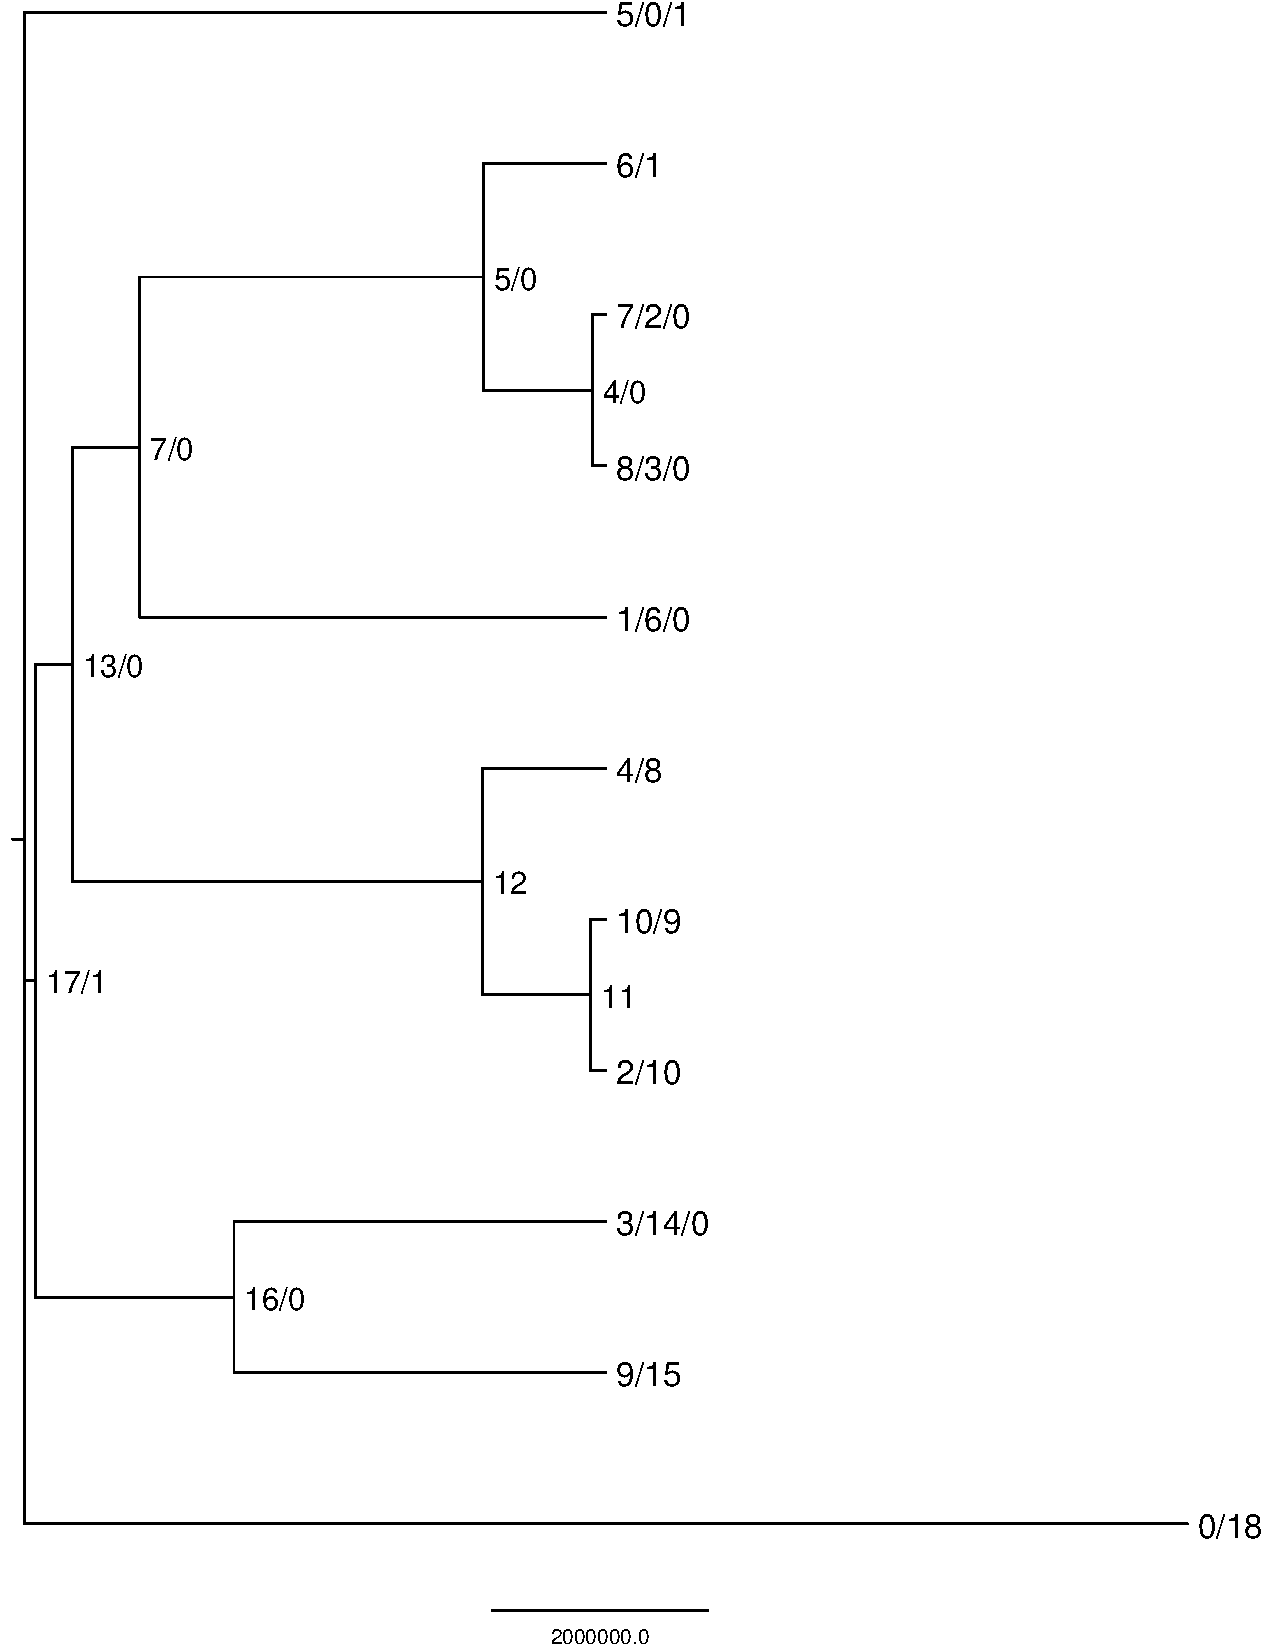
\includegraphics[scale=0.6]{54_1_taxon_tree_with_score.pdf}
  \caption{model condition - model.10.5400000.0.000000037 - Replicate R1 - Fixed quintet}
\end{figure}

 U = [955, 23, 22, 0, 0, 0, 0, 0, 0, 0, 0, 0, 0, 0, 0]
 \clearpage
  {\bf  model condition - model.10.5400000.0.000000037 - Replicate R3 - Fixed quintet } \\
 
\begin{figure}[h]
  \centering
  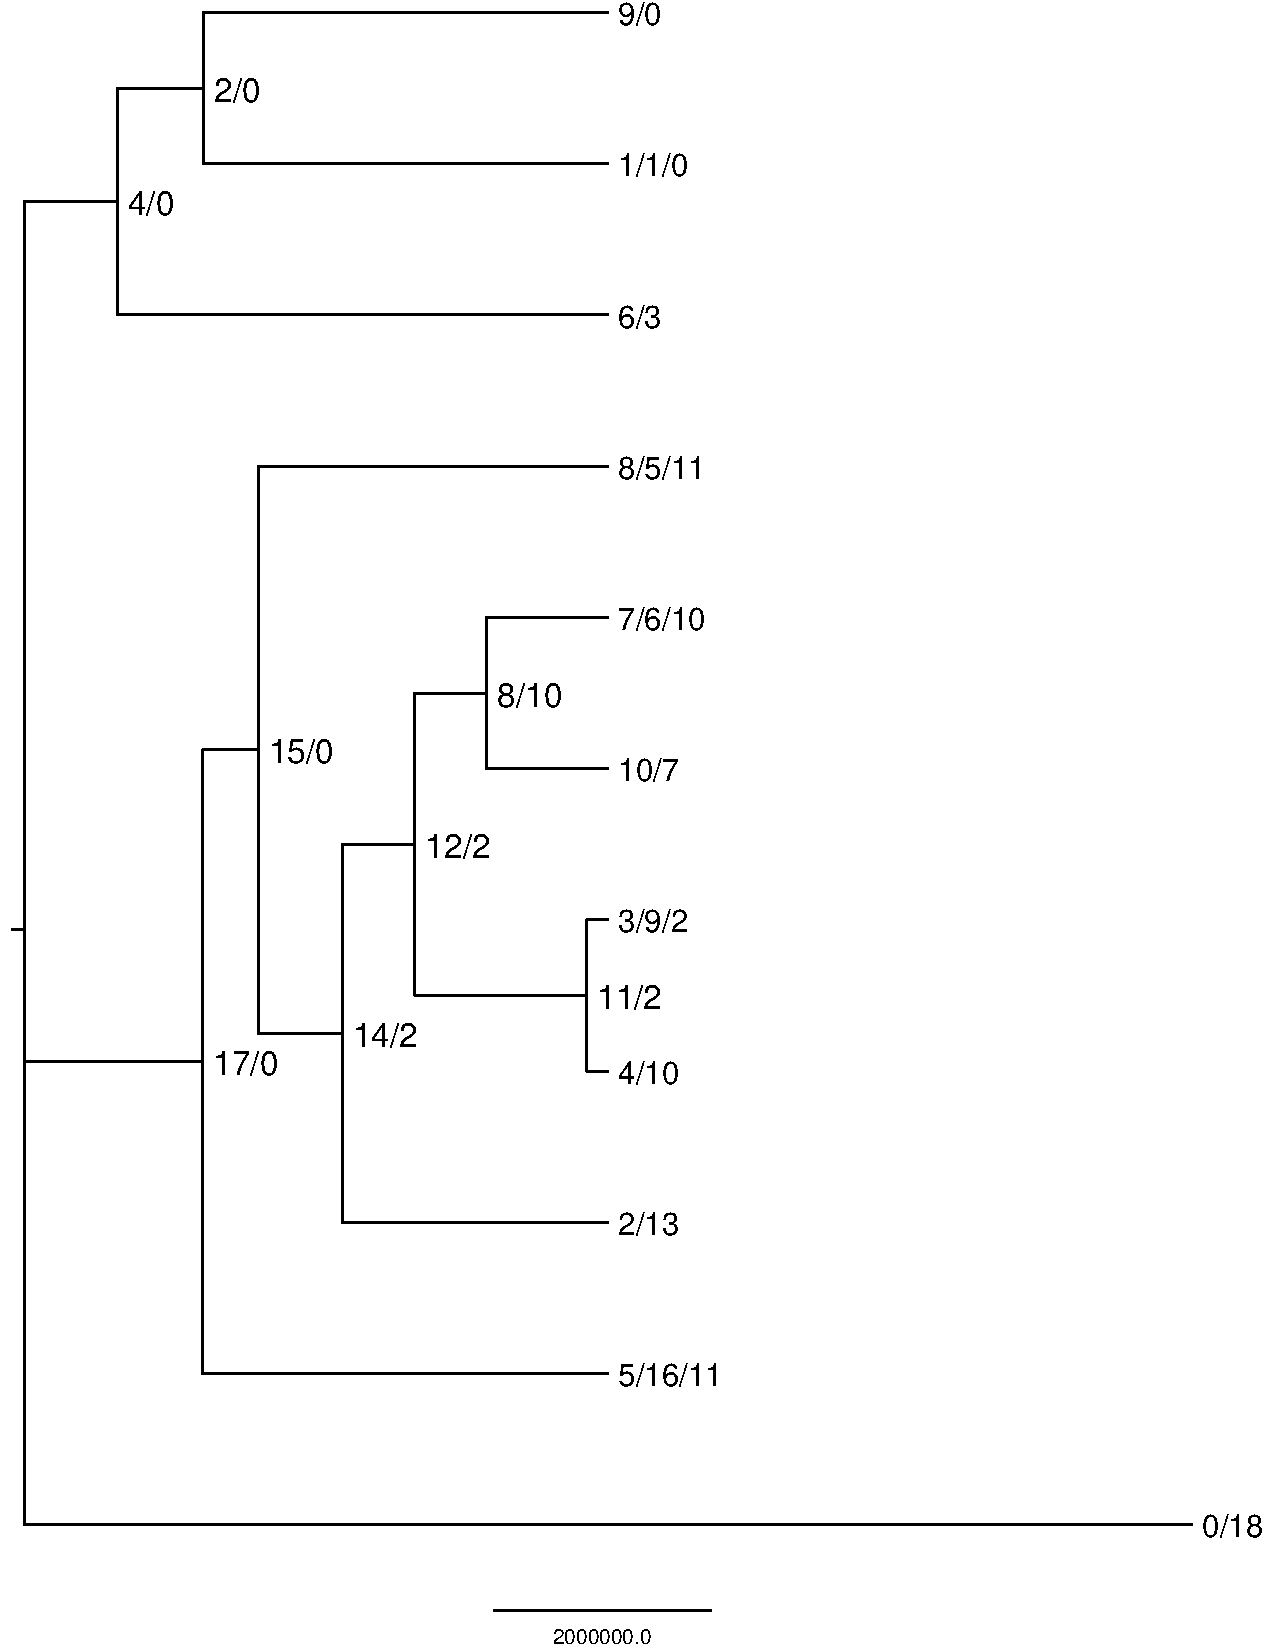
\includegraphics[scale=0.6]{54_3_tree_with_score.pdf}
  \caption{model condition - model.10.5400000.0.000000037 - Replicate R3 - Fixed quintet}
\end{figure}

 
 
 U = [799, 83, 92, 14, 0, 2, 0, 0, 2, 0, 0, 2, 6, 0, 0]

 \clearpage
  {\bf  model condition - model.10.1800000.0.000000111 - Replicate R1 - Fixed quintet } \\
 

\begin{figure}[h]
  \centering
  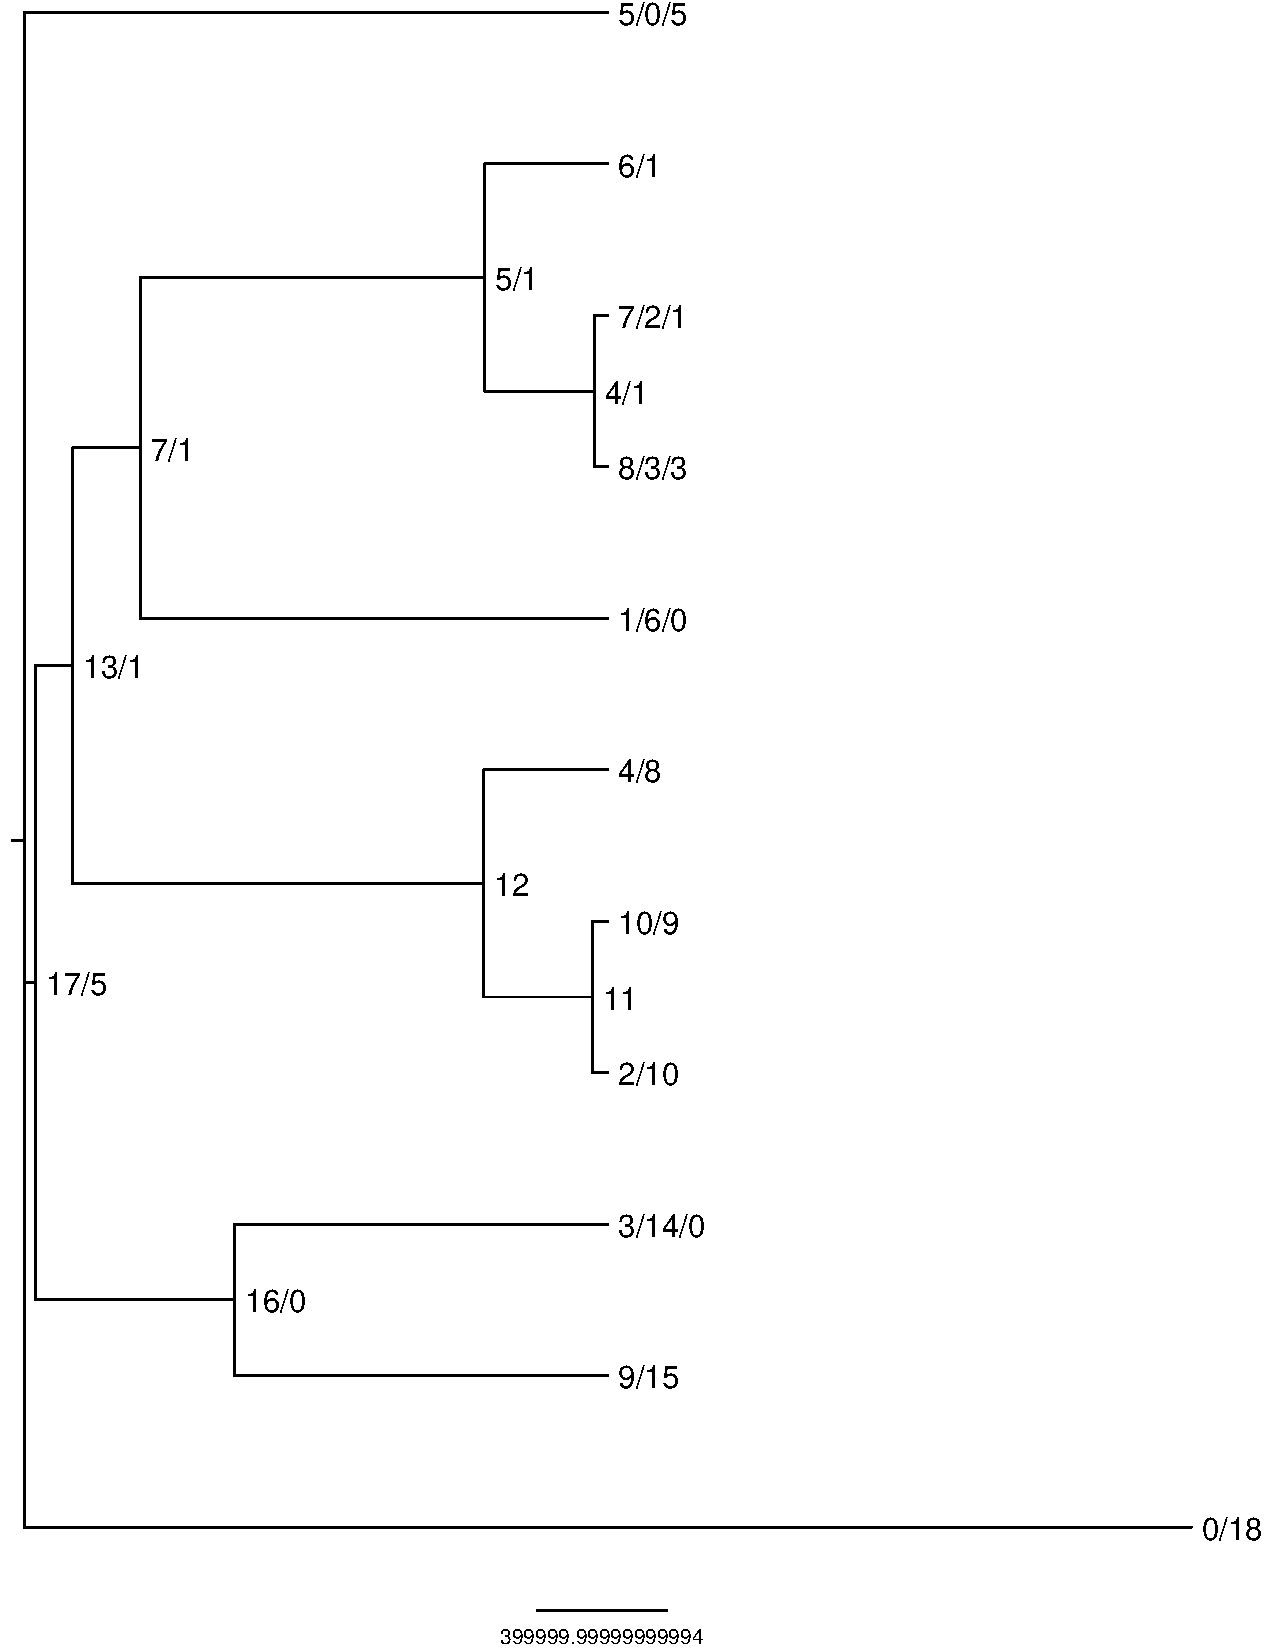
\includegraphics[scale=0.6]{18_1_10_taxon_tree_with_score.pdf}
  \caption{model condition - model.10.1800000.0.000000111 - Replicate R1 - Fixed quintet}
\end{figure}


 U = [681, 155, 153, 2, 3, 1, 0, 0, 1, 0, 0, 0, 4, 0, 0]

 \clearpage
  {\bf  model condition - model.10.1800000.0.000000111 - Replicate R2- Fixed quintet } \\
 
\begin{figure}[h]
  \centering
  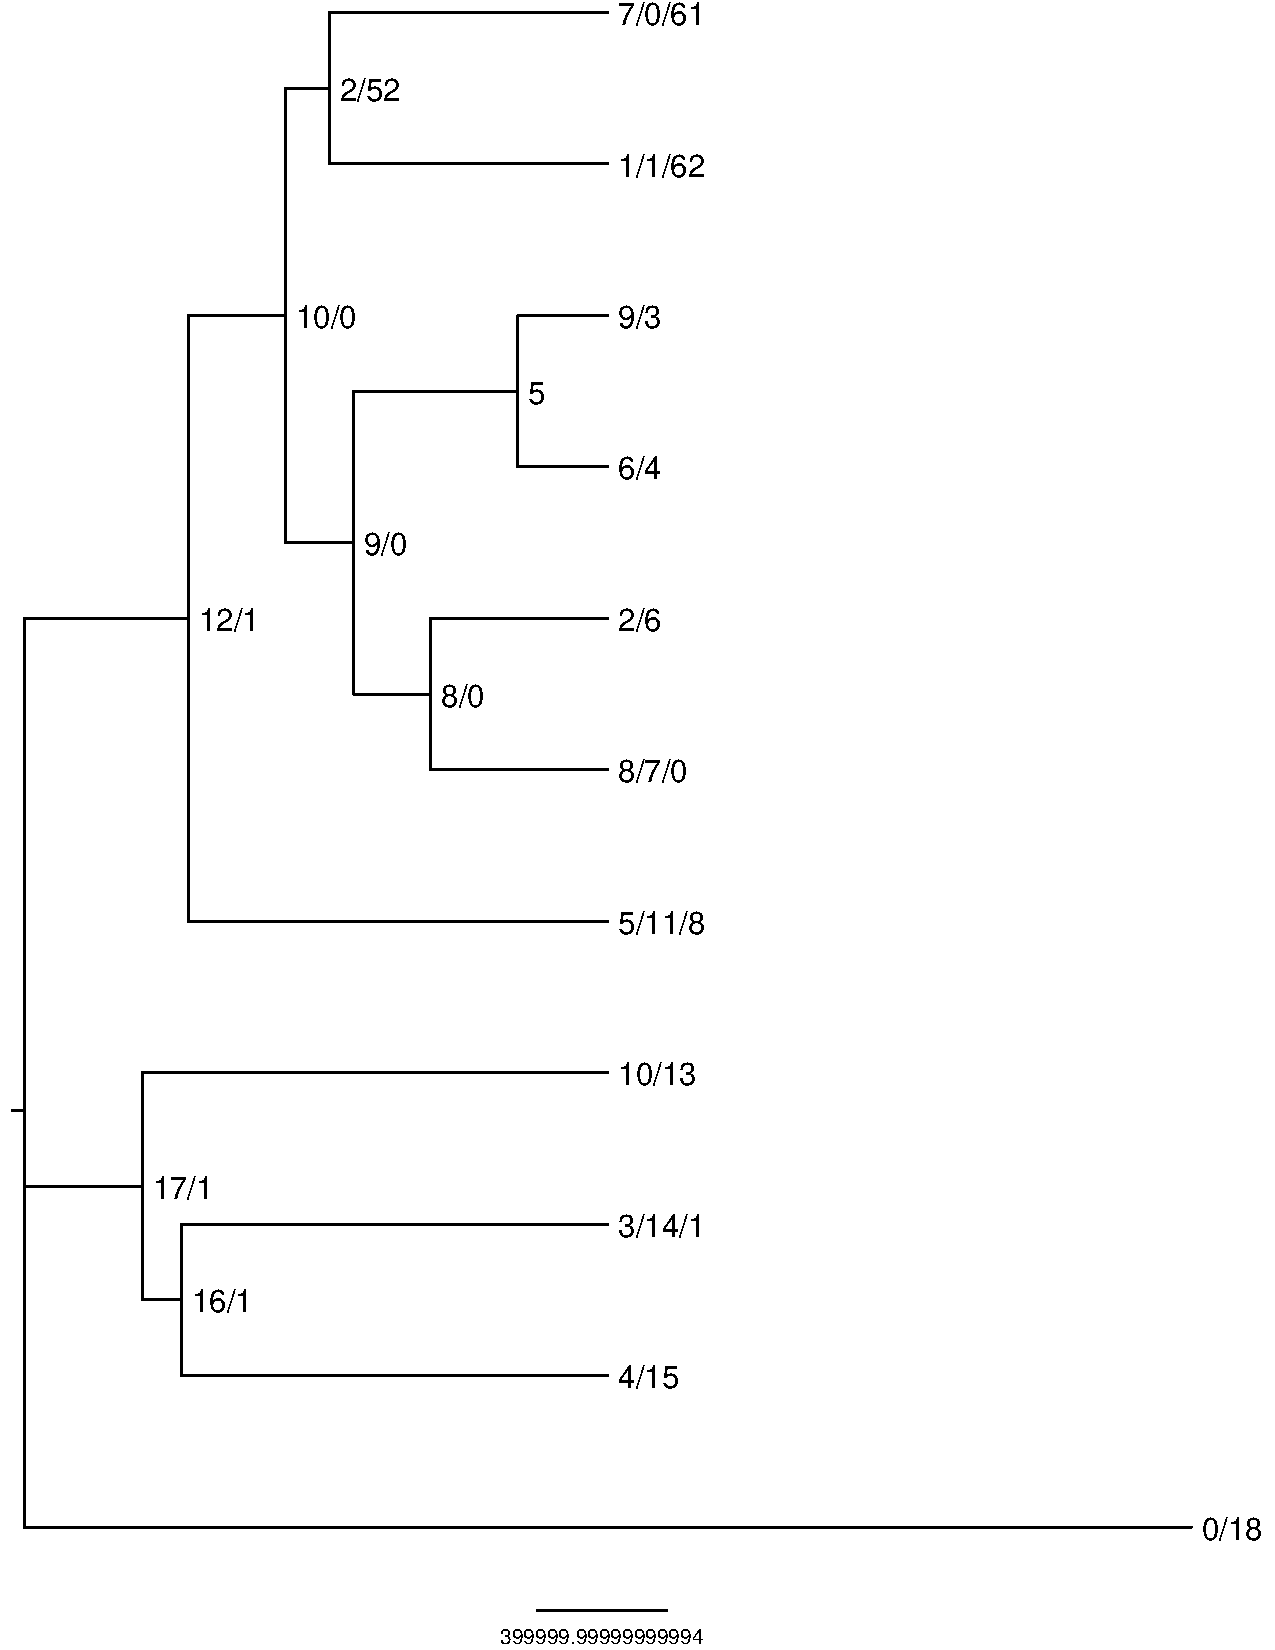
\includegraphics[scale=0.6]{18_2_10_taxon_tree_with_score.pdf}
  \caption{model condition - model.10.1800000.0.000000111 - Replicate R2- Fixed quintet}
\end{figure}
 
 U = [302, 93, 92, 131, 55, 63, 1, 3, 59, 2, 4, 45, 136, 7, 7]
 
   
  \clearpage
  {\bf  model condition - model.10.600000.0.000000333 - Replicate R1 - Fixed quintet } \\
 
\begin{figure}[h]
  \centering
  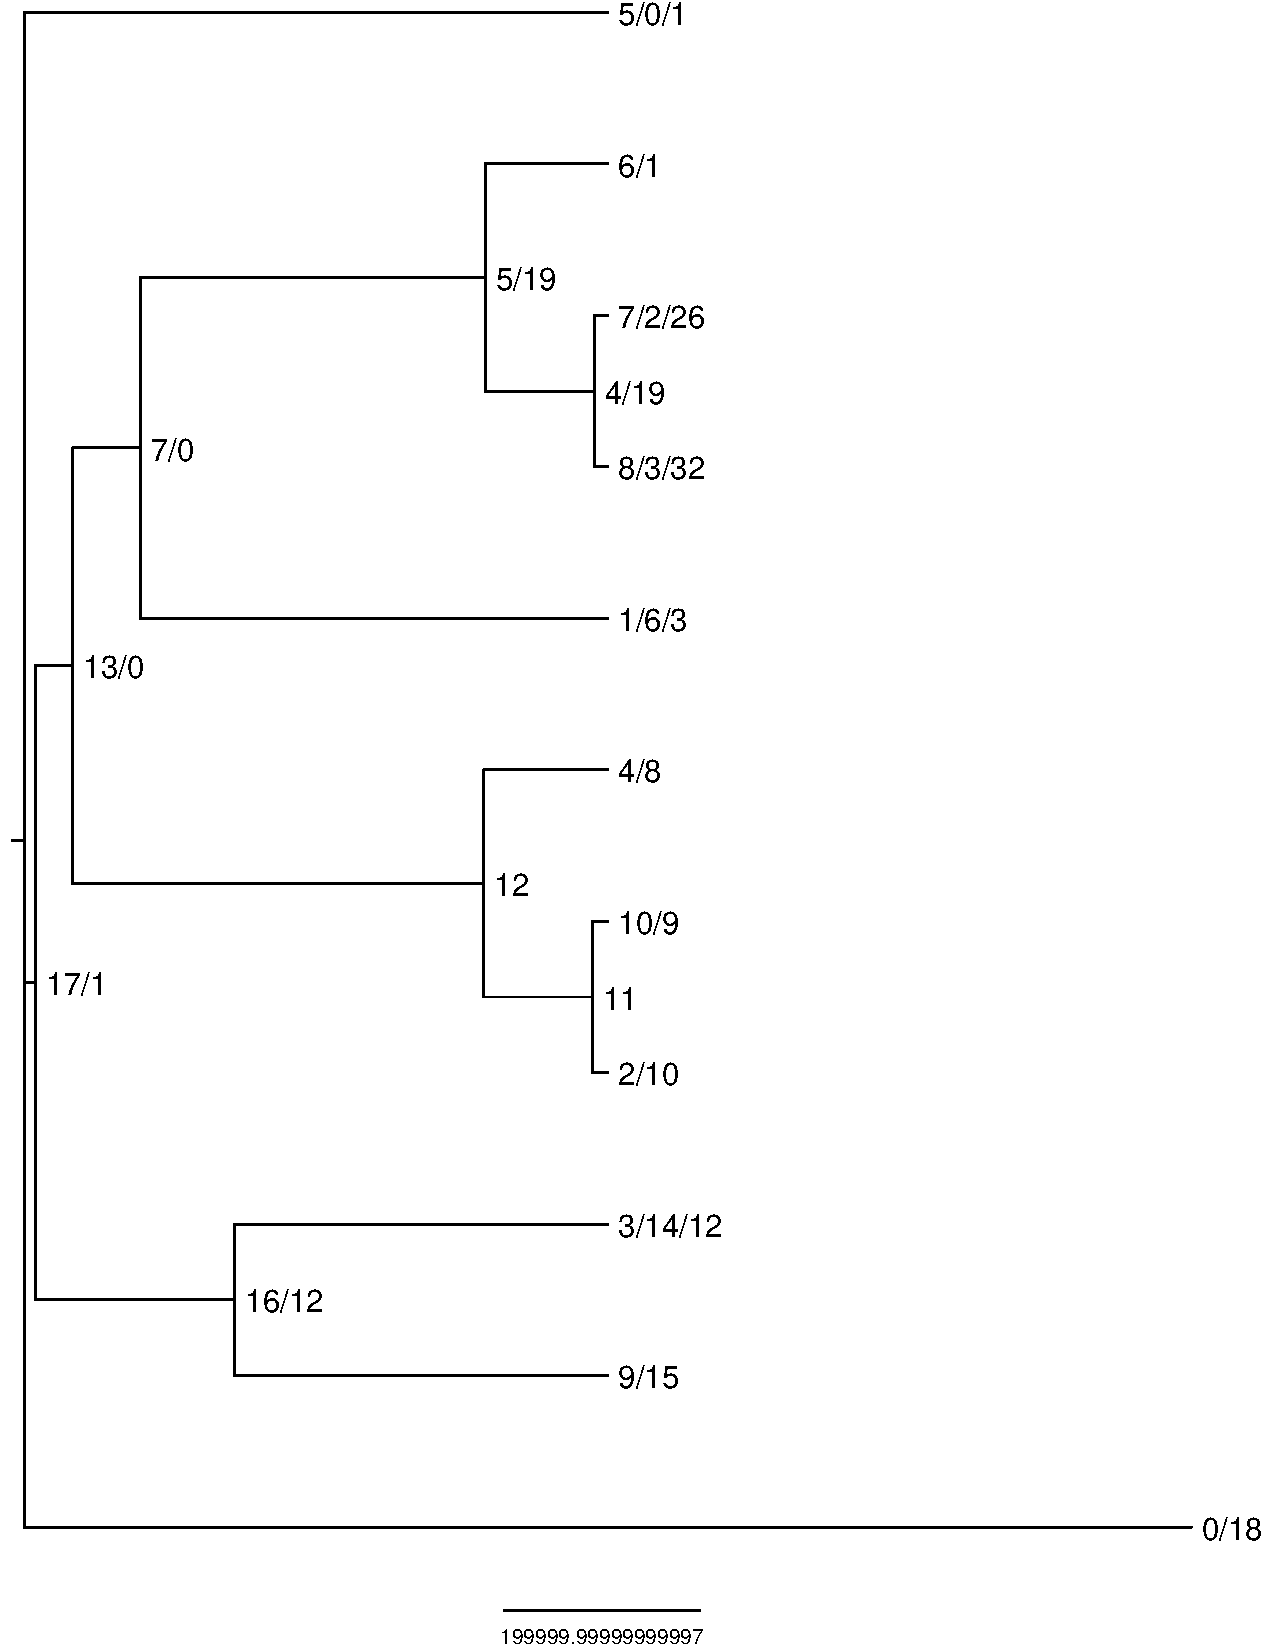
\includegraphics[scale=0.6]{60_1_10_taxon_tree_with_score.pdf}
  \caption{model condition - model.10.600000.0.000000333 - Replicate R1 - Fixed quintett}
\end{figure}
 
 U = [362, 203, 202, 28, 24, 32, 10, 12, 28, 6, 10, 29, 38, 7, 9]


 
\end{document}